%%% template.tex
%%%
%%% This LaTeX source document can be used as the basis for your technical
%%% paper or abstract.

%%% The parameter to the ``documentclass'' command is very important.
%%% - use ``review'' for content submitted for review.
%%% - use ``preprint'' for accepted content you are making available.
%%% - use ``tog'' for technical papers accepted to the TOG journal and
%%%   for presentation at the SIGGRAPH or SIGGRAPH Asia conference.
%%% - use ``conference'' for final content accepted to a sponsored event
%%%   (hint: If you don't know, you should use ``conference.'')

\documentclass[tog]{acmsiggraph}

\usepackage[normalem]{ulem}
\usepackage{bm}
\usepackage{enumitem}
\usepackage{algorithm}
\usepackage[noend]{algpseudocode}

%%% Make the ``BibTeX'' word pretty...

\def\BibTeX{{\rm B\kern-.05em{\sc i\kern-.025em b}\kern-.08em
    T\kern-.1667em\lower.7ex\hbox{E}\kern-.125emX}}

%%% Used by the ``review'' variation; the online ID will be printed on 
%%% every page of the content.

\TOGonlineid{45678}

%%% Used by the ``preprint'' variation.

\TOGvolume{0}
\TOGnumber{0}

\title{Real-Time tearing and fracturing}

\author{Myriam Beauvais\thanks{e-mail:myriam.beauvais@mail.mcgill.ca} \\ ID 260760034 \\COMP-559, Fundamentals of Computer Animation}
\pdfauthor{Stephen N. Spencer}

\keywords{tearing, fracturing, deformation, animation}

\begin{document}
\setlist[0]{noitemsep}

%%% This is the ``teaser'' command, which puts an figure, centered, below 
%%% the title and author information, and above the body of the content.

 \teaser{
   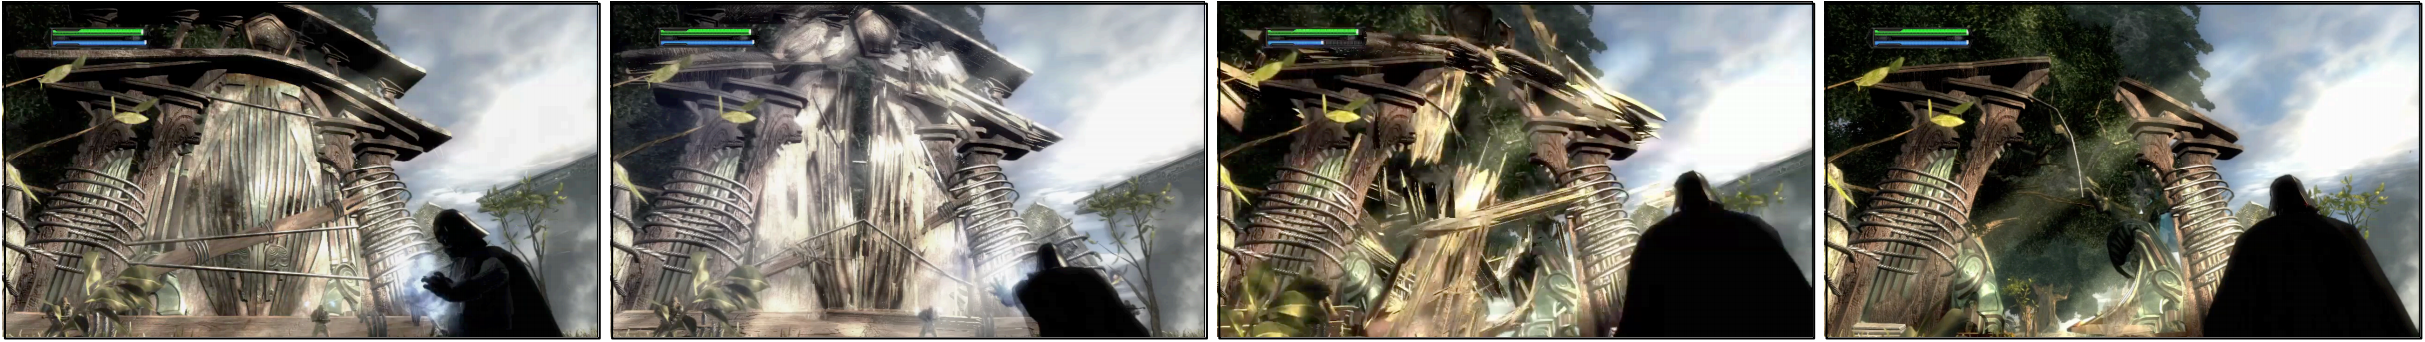
\includegraphics[height=0.98in]{images/Teaser}
   \caption{Star Wars: The Force Unleashed game content and screenshots courtesy of LucasArts, a division of Lucasfilm Entertainment Company Ltd. \copyright 2009 Lucasfilm Entertainment Company Ltd. or
Lucasfilm Ltd. All rights reserved. Image taken from Parker and O'Brien, 2009}
 }

\maketitle

\copyrightspace

\section{Abstract}
This project is an attempt at replicating \cite{Obrien:1999:GMA}'s cracking and fracturing work in Unity 3D, leveraging its \textit{PhysX} physics engine. The work relies on calculating stress tensors for the different triangles of a mesh and analyse the corresponding forces to assess if the object will fracture and where and how it will do so. Based on the latter information, remeshing of the object is executed. For simplification, our implementation only handles 2D meshes, allowing to do the tensor calculations on triangles instead of on tetrahedrons. 

\section{Introduction}
A lot of different objects, when under some persistent and or increasing forces, will end up getting distorted and breaking apart. Because virtual objects are often put in such situations in video games, movies or simulations, addressing this topic is very pertinent and interesting in order to recreate realistic sequences.  

The project presented is the implementation of an interactive application allowing for deformation, tearing and fracturing of meshes in real-time, according to the method described in \cite{Obrien:1999:GMA}. 

The initial proposal was to implement the work of \cite{Parker:2009:RTD}. While the overall work adds to the fracturing algorithm, the section specifically dedicated to fracturing is very similar to  \cite{Obrien:1999:GMA}'s method except that they don't replicate tetrahedrons while remeshing. To focus more on the fracturing algorithm, we worked on \cite{Obrien:1999:GMA}'s method exclusively. 

\section{Related Work}
Fracturing of objects is a well studied topic for which many approaches were proposed. While many models are based of physically based methods, some also proposed less physically perfect but visually appealing techniques such as procedural algorithms. 

This work is mainly based of the algorithm described by \cite{Obrien:1999:GMA} which models a fracture using a separation tensor, calculated over the volume of a mesh. They calculate the separation tensors of a point based on the force tensors of connecting tetrahedral elements. 

\cite{Parker:2009:RTD} Propose improvements upon \cite{Obrien:1999:GMA}, optimizing and adapting its work, using many ideas proposed in the literature, in order to provide a system that simulates fractures and deformations in a real-time context.

\section{Technical details}
As this project is mainly the implementation of \cite{Obrien:1999:GMA} for a 2D mesh in Unity, most of the technical details revolves around adapting the algorithm to the Unity context and how to leverage Unity's physics Engine to handle collisions and most physics aspects unrelated directly to fracturing. To understand better the work that has been made, we'll describe the modifications made to \cite{Obrien:1999:GMA}'s algorithm and the technical aspects needed to implement it in Unity.

\subsection{Fracturing}
\label{sec:Fracturing}
Most of the calculations made in this project are in order to compute the separation tensor. Using the latter gives information about if a fracture should happen, at which point and how it will spread. Based on a simplification of \cite{Obrien:1999:GMA}'s fracturing algorithm, we first divide our 2D mesh into triangle elements, each defined by three nodes. The latter have a position in material coordinates, $\pmb{m}$ - which in Unity corresponds to the mesh's \textit{GameObject}'s local space - and a position and a velocity in world space, $\pmb{p}$ and $\pmb{v}$. 

We define three matrices $\mathbf{P}$, $\pmb{V}$ and $\pmb{\beta}$ as

\begin{gather}
\pmb{P} = [
\begin{matrix}
\pmb{p}_{[1]} & \pmb{p}_{[2]} & \pmb{p}_{[3]}
\end{matrix}]\\
\pmb{V} = [
\begin{matrix}
\pmb{v}_{[1]} & \pmb{v}_{[2]} & \pmb{v}_{[3]}
\end{matrix}]\\
\pmb{\beta} = [
\begin{matrix}
\pmb{m}_{[1]} & \pmb{m}_{[2]} & \pmb{m}_{[3]}
\end{matrix}]^{-1} .
\end{gather}

These are used to build two $3 \times 3$ tensors; the Green's strain tensor, $\pmb{\epsilon}$ and the strain rate tensor $\pmb{\nu}$ defined by 

\begin{gather}
\epsilon_{ij} = \left(\frac{\partial \pmb{x}}{\partial u_i} \cdot \frac{\partial \pmb{x}}{\partial u_j}\right) - \delta_{ij}, \\
\nu_{ij} = \left(\frac{\partial \pmb{x}}{\partial u_i} \cdot \frac{\partial \pmb{\dot{x}}}{\partial u_j}\right) +  \left(\frac{\partial \pmb{\dot{x}}}{\partial u_i} \cdot \frac{\partial \pmb{x}}{\partial u_j}\right)
\end{gather}
with $\pmb{u} = [u, v, w]^T$, a location in the material coordinate, $\pmb{x(u)} = [x,y,z]^T$ a function mapping the material coordinates to world coordinates and $\delta_{ij}$ being the Kronecker delta : 
\begin{gather}
\delta_{ij} = \begin{cases} 
1 : i = j\\
0 : i \neq j.
\end{cases}
\end{gather}

The tensors can be easily computed using 
\begin{gather}
\frac{\partial \pmb{x}}{\partial u_i} = \pmb{P \beta \delta}_i\\
\frac{\partial \pmb{\dot{x}}}{\partial u_i} = \pmb{V \beta \delta}_i
\end{gather}

with

\begin{gather}
\pmb{\delta}_i = [\begin{matrix}
\delta_{i1} & \delta_{i2} & \delta_{i3}
\end{matrix}]^T.
\end{gather}

We then calculate the elastic stress $\pmb{\sigma}^{(\epsilon)}$, function of the strain, the material's rigidity $\mu$ and dilation $\lambda$ and the viscous stress $\pmb{\sigma}^{(\nu)}$, function of the strain rate and two parameters $\phi$ and $\psi$ :

\begin{gather}
\pmb{\sigma}_{ij}^{(\epsilon)} = \sum_{k =1}^3 \lambda \epsilon_{kk} \delta_{ij} + 2\mu \epsilon_{ij}\\
\pmb{\sigma}_{ij}^{(\nu)} = \sum_{k =1}^3 \phi \nu_{kk} \delta_{ij} + 2\psi \nu_{ij}.
\end{gather} 

The total resulting stress $\pmb{\sigma}$ is the sum of the elastic and the viscous stress, $\pmb{\sigma} = \pmb{\sigma^{(\epsilon)}} + \pmb{\sigma^{(\nu)}}$. The stress tensor is then decomposed into a tensile component, $\pmb{\sigma}^+$, and a compressive component, $\pmb{\sigma}^-$ : 

\begin{gather}
\pmb{\sigma}^+ = \sum_{i=1}^3 \max (0, \mathrm{v}^i(\pmb{\sigma})) \ \pmb{\mathrm{m}}(\pmb{\hat{\mathrm{n}}}^i(\pmb{\sigma}))\\
\pmb{\sigma}^- = \sum_{i=1}^3 \min (0, \mathrm{v}^i(\pmb{\sigma})) \ \pmb{\mathrm{m}}(\pmb{\hat{\mathrm{n}}}^i(\pmb{\sigma})),
\end{gather}

where $\mathrm{v}^i(\pmb{\sigma})$, the \textit{i}th eigenvalue of $\pmb{\sigma}$, $\pmb{\hat{\mathrm{n}}}^i(\pmb{\sigma})$ the corresponding unit eigenvector and 

\begin{gather}
\pmb{\mathrm{m}(a)} =
\begin{cases}
\pmb{aa}^T/|\pmb{a}| & : \pmb{a} \neq 0\\
0 & : \pmb{a} = 0
\end{cases}.
\end{gather}


This allows to compute the tensile and compressive forces exerted on a particle $i$ by one triangle, and compute it for all triangles in the mesh : 

\begin{gather}
\label{eqfp} \pmb{f}_{[i]}^{+} = -\frac{area}{2}\sum_{j = 1}^3 \pmb{p}_{[j]}\sum_{k=1}^3 \sum_{l=1}^3 \pmb{\beta}_{jl} \pmb{\beta}_{ik} \pmb{\sigma}_{kl}^{+}\\
\label{eqfm} \pmb{f}_{[i]}^{-} = -\frac{area}{2}\sum_{j = 1}^3 \pmb{p}_{[j]}\sum_{k=1}^3 \sum_{l=1}^3 \pmb{\beta}_{jl} \pmb{\beta}_{ik} \pmb{\sigma}_{kl}^{-}.
\end{gather}

Having the sets of tensile and compressive forces applied by each elements attached to a point, $\{\pmb{f}^+\}$ and $\{\pmb{f}^-\}$, it is possible to calculate the separation tensor :

\begin{gather}
\pmb{\zeta} = \frac{1}{2}\left(-\pmb{\mathrm{m}}(\pmb{f}^+) + \sum_{\pmb{f} \in {\pmb{f}^+}} \pmb{\mathrm{m}}(\pmb{f}) +\pmb{\mathrm{m}}(\pmb{f}^-) - \sum_{\pmb{f} \in {\pmb{f}^-}} \pmb{\mathrm{m}}(\pmb{f}) \right).
\end{gather}

A fracture is happening at the point evaluated if the largest positive eigenvalue $\mathrm{v}^+$ of $\pmb{\zeta}$ is greater than $\tau$, the material toughness. Taking the corresponding eigenvector $\mathrm{\pmb{\hat{n}}}^+$, we get the fracture plane's normal.

These calculations are all exactly the same as described in \cite{Obrien:1999:GMA} except for the dimensions of the matrices $\pmb{P}$, $\pmb{V}$ and $\pmb{\beta}$ that are adapted for three nodes instead of four and the number of iterations of the first sum in \eqref{eqfp} and \eqref{eqfm} that has also been brought down to three. 

\subsection{Implementation}
The methods and algorithms described were implemented in Unity3D with the use of custom scripts. The project's setup is a scene composed of three \textit{GameObject}s; a \textit{Camera}, a \textit{Light} and a \textit{Scene Manager}. To allow interaction with the objects, a basic First Person Camera behaviour was implemented and added to the \textit{Camera object}. The \textit{Scene Manager} object has two \textit{Script Components}. The first one describes the creation of the test scene, with an object that can be fractured and the second one allows for picking and dragging objects in the scene using an external force. 

\subsection{Interactions}
As this project is based of an empty 3D scene in Unity, we added some simple interaction options for the purpose of this project. Basic first person controls were added to the scene's camera. 

\begin{itemize}
\setlength\itemsep{0em}
\item $\uparrow$ : Move Forward
\item $\downarrow$ : Move Backward
\item $\leftarrow$ : Move Left
\item $\rightarrow$ : Move Right
\item $\left[alt\right]$ + Click : Rotate 
\end{itemize}

Interaction with the objects is based on a ray cast algorithm slightly modified from \cite{Drag}'s. A ray starting from the mouse's position and triggered by a click, tells whether an object was selected or not. If so, an external force is applied on the latter, defined by a vector between the initial click point and the updated mouse's position. Proceeding with a force instead of a simple drag and drop allows for the spring system to be influenced by the displacement of the selected object. 

\subsubsection{Test Scene Creation}
The test scene has only one object which can be fractured and a plane. The breakable object is forced to be a plane itself for simplification purpose, and it's size can be fixed by a parameter available to the user (\textit{MeshPoints}). The decision of limiting the shape of the object to a plane allows to treat it as a simple 2D mesh and implement \cite{Obrien:1999:GMA}'s fracturing algorithm using triangles instead of tetrahedrons. 

\subsubsection{Fracturable Objects}
A fracturable object is made of a set of particles that are managed by Unity's Physics Engine. Those particles are linked together with horizontal, vertical and diagonal springs. The mesh of the object is bound to those particles with each of it's vertices mapped on a corresponding particle. Using the vertex and the index buffers of the mesh, it's possible to define the set of triangles that constitutes it. Since calculations are mostly made triangle-wise, we define a structure that represent one single triangle, referring to the particles that constitutes it. All tensor computations are then made within this structure. The separation tensor is calculated within each particles, using force and stress information sent by all triangles connected to the particle. 

\begin{figure}[ht]
  \centering
  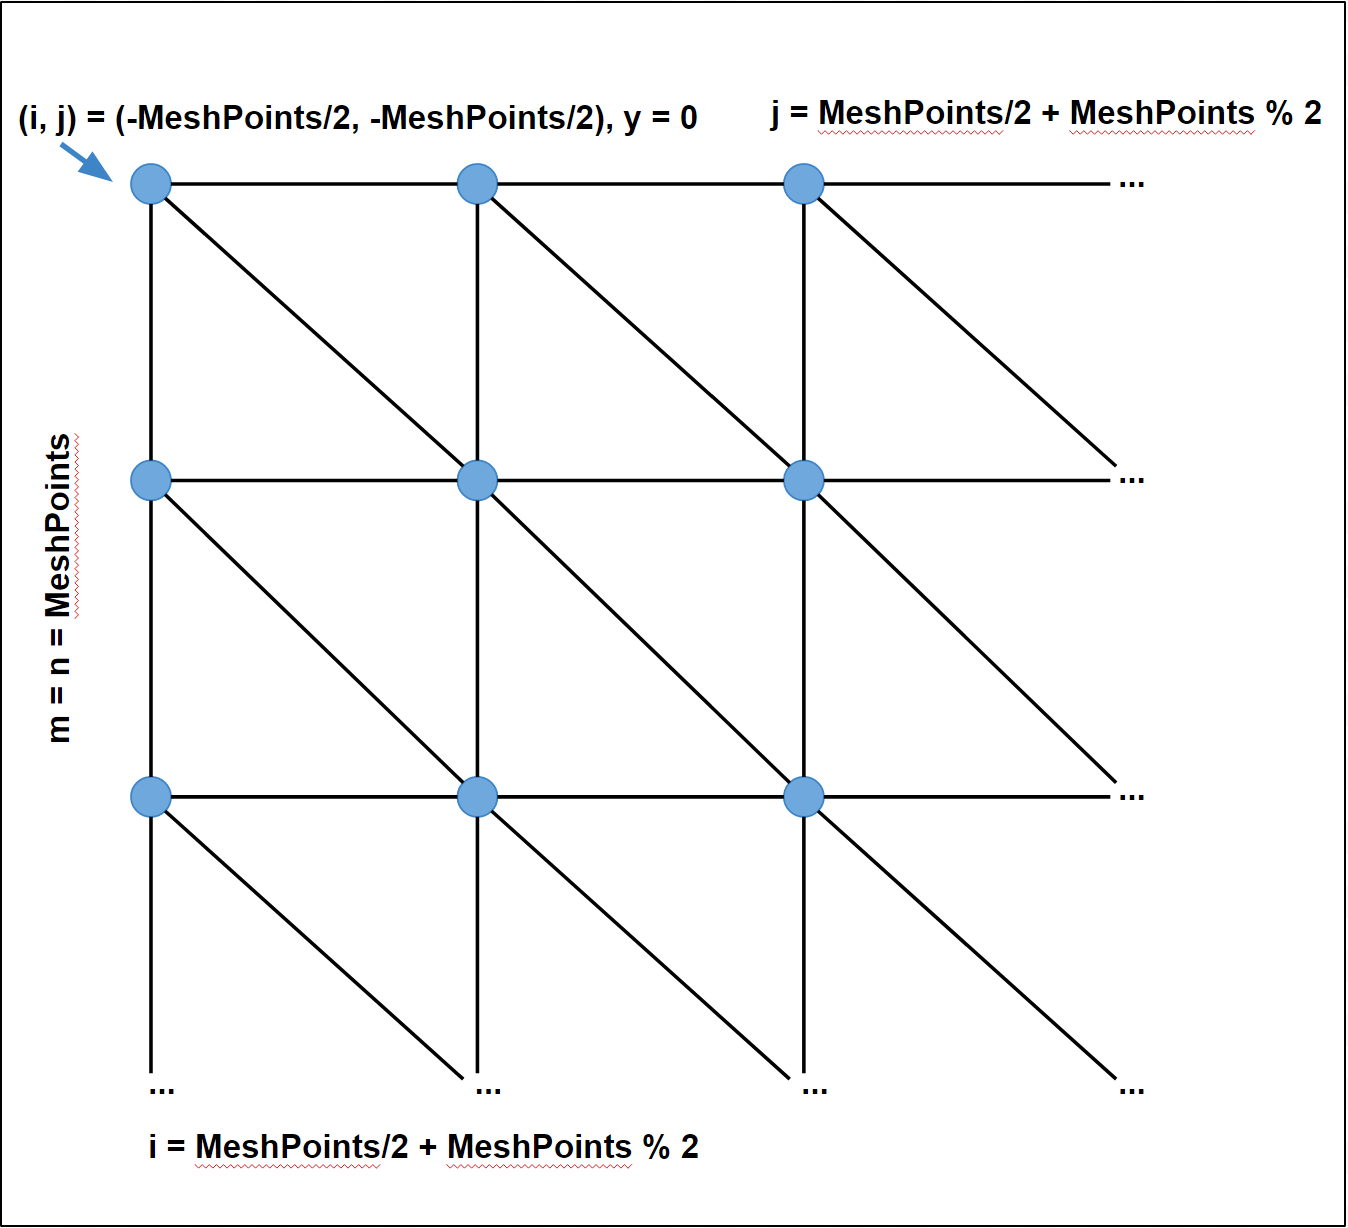
\includegraphics[width=2.5in]{images/MeshDescription}
  \caption{Structure of the implemented Mesh}
  \label{fig:meshdescription}
\end{figure}

The figure \ref{fig:meshdescription} visually present the relation between the different particles, the springs and the triangles. The dimensions of the 2D object are controlled by a single parameter \textit{MeshPoints} that controls how many points on each axis there would be, forming a square shaped plane. The object's particles coordinates vary in $x$ and $z$ between $[-MeshPoints/2, MeshPoints/2 + MeshPoints\% 2]$ and the $y$ coordinates are set to 0. 

\subsubsection{Joints between particles}
A challenging part of this project was to define the joints between the particles. three different joints were tested: Spring Joints, Hinge Joints and custom scripted springs. 

Spring joints is the most intuitive choice of structure as we are looking for very stiff springs to attach all particles together. After trying a lot of different parameters, it is difficult to get the springs to not only act stiff but to properly transmit force to the linked rigid bodies in our particular setup. 

We then tried Hinge Joints. Using this structure along with a spring gave good visual results and a stiffer structure. However, it wasn't satisfying, as this joint impose motion restriction that doesn't apply to our context.

The joints that are used in the final project are springs defined by a custom script. Connecting all particles with these allows for enough deformation within the material to calculate a difference in velocities between two particles that would induce a fracture. The chosen stiffness for all springs is $k = 800$ and the damping is $c = 10$. This happened to be a good compromise between stiffness and stability. Unity's solver gets unstable when the stiffness of the springs is too high and having the parameter $k$ to a even higher value in order to represent tougher materials would make the system blow up. For using those joints, we also added a drag of 5 to the rigid bodies, which were otherwise behaving as frictionless objects.  

Unity's physics solver parameters have been set to the maximum number of iterations and the accuracy of the resulting velocity after a bounce was also augmented $Default\ solver\ iteration = 255$ and $Default\ solver\ velocity = 15$. This lowers the overall performance but as we are only testing for one object, the former is not an issue.

\subsubsection{Remeshing}
The eigenvector returned by the separation tensor corresponds to the normal of the separation plane. Once a fracture is found, we go through all triangles of the mesh to verify if they are connected to the point of fracture and then if they intersect with the separation plane, using \cite{Inters}'s algorithm. Each points of connected triangles are mapped to a side of another of the plane using a boolean value for which \textit{false} means a node is on the negative side of the plane whereas \textit{true} means the node is on the positive side. We avoid setting the side of a node two times by keeping another boolean value that informs if the calculations have already been made for the particle. 

\begin{figure}[ht]
  \centering
  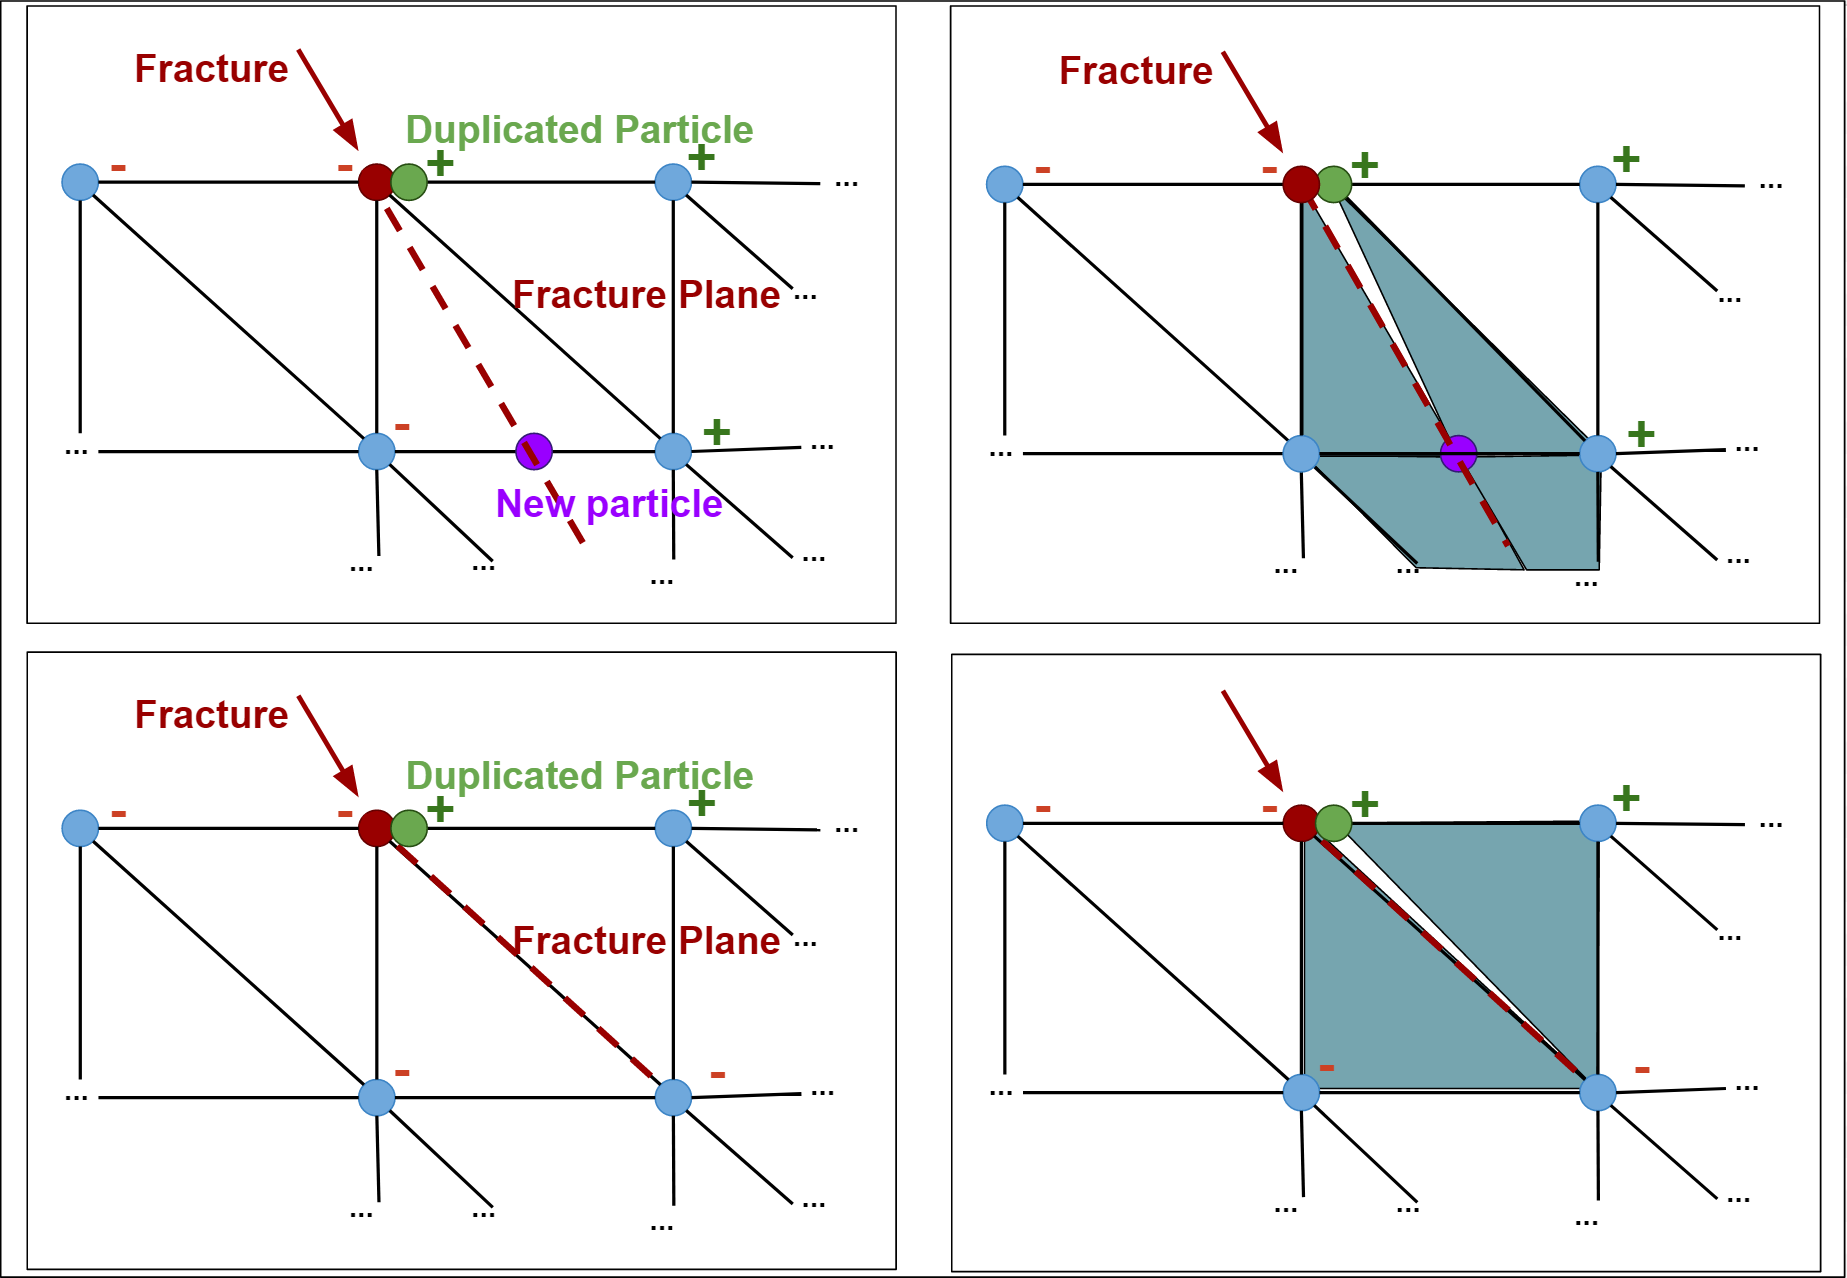
\includegraphics[width=3.5in]{images/fractures}
  \caption{Remeshing Steps and triangle creation}
  \label{fig:remeshing}
\end{figure}

If the plane intersects with a triangle, the latter is separated along the intersection line. First, the particle where the fracture happens is duplicated. Then we test if the plane goes through an already existing node. If so, we undergo simple reassignment of springs between the duplicated node, the original node itself and the existing node on the plane. Otherwise, a new particle is created at the intersection point. This implies a more complex spring reassignment step, as the springs on which the new node is positioned needs to be divided in two and new connections needs to be created to conserve the mesh's integrity. The resulting remeshing is presented in figure \ref{fig:remeshing}, where are illustrated the fracture plane, the original and the duplicated particles, the new particle in the first case and the sides (plus or minus) of each nodes connecting to the point where the fracture initiates. In turquoise is shown the affected triangles and the new ones created. 

Based on the new spring connections, we then update the mesh fully, redefining new triangles and indices. 

\section{Results and Discussion}

DESCRIBE RESULTS

Even though there is only one \textit{FracMesh} object for the whole scene, we are able to handle fully divided meshes. Because of the independent handling of the particles, the two sections will physically and visually act as two separate meshes. 

Even though many eigenvalues of the separation tensors are greater than the material's toughness, our algorithm only handles one separation plane, contrary to what is proposed by \cite{Obrien:1999:GMA}.

An accessible improvement to this project would be to extend it to full 3D shapes, like described in \cite{Obrien:1999:GMA}. The fracturing algorithm and calculations are pretty much the same except for the few tweaks made to use three nodes instead of four as described in section \ref{sec:Fracturing}. The remeshing is probably the most challenging part of this extension and would likely account for the biggest amount of work to be done. 

In order to manage a larger range of materials, it would be useful to implement a Linear Backward Euler solver in Unity. It would imply getting rid of most of the used features of the \textit{PhysX} Engine and recoding them, inserting the solver calculations into a \textit{Monobehaviour} class' \textit{Update} function. Such an extension to the current project would allow to handle a higher stiffness on the springs and would guarantee much more stability of the system in general. 

Finally, the collision detection is only enabled in the project on the rigid bodies. It would be useful to improve the overall project with collision detection on the mesh with itself, to avoid particles to inter-penetrate the mesh. 

\section{Conclusion}

In this project, we first built a simple scene within Unity and implemented basic interaction options. We defined a plane creation sequence that automatically create a fracturable object, constituted of particles, springs and triangles. A mesh is then mapped on top of the particles using their positions as the vertices' coordinates. Once all components are created, we undergo fracture testing at each update of the scene using \cite{Obrien:1999:GMA} algorithm, modified for triangular elements instead of tetrahedral ones. If a point should be fracturing, we calculate the fracture plane's normal and for each triangles connected to the point, we verify if they intersects with the plane. If so, we compute at which point the intersection happens. We also attribute a plane side to each particles connected to the point of fracture which helps proper remeshing. An triangle intersecting the plane is divided along the intersection line. Springs are consequently redistributed in such a way to take account of the new mesh's shape and finally the mesh's updated.

Latter improvement of this work made many optimizations, improved mesh deformation handling, allowed more precise tearing and fracturing of different material, proposed procedural approaches, etc.  



%%\section{Figures and Tables and Captions}

%%Figures and tables can span one or both columns. Captions for figures
%%should be centered underneath the figure. Captions for tables should
%%be centered above the table.

%%\begin{table}[ht]
%%  \centering
%%  \caption{A simple table.}
%%  \begin{tabular}{|r|l|}
%%    \hline
%%    7C0 & hexadecimal \\
%%    3700 & octal \\ \cline{2-2}
%%    11111000000 & binary \\
%%    \hline \hline
%%    1984 & decimal \\
%%    \hline
%%  \end{tabular}
%%\end{table}
  
%%Please use 9-point bold serif type for the caption title, and 9-point
%%serif type for the caption text (both on 10-point line spacing).

%\section{Citations and References}
%
%\subsection{Citations}
%
%The SIGGRAPH citation format is the ``author year''
%format~\cite{Pellacini:2005:LAH}. The year is separated from the
%author by a single space~\cite{yee:2000:ssa}. Two authors are
%separated by the word ``and''~\cite{parke:1996:CFA}. More than two
%authors are represented by the primary author and ``et al.''~\cite{levoy:2000:TDM}.
%
%Multiple citations at a single point in the content are separated by
%semicolons~\cite{levoy:2000:TDM,sako:2001:SSB}.
%
%When the last name of the cited author is part of the text, it may be
%omitted from the citation: ``\ldots as shown in Fedkiw et
%al.~\shortcite{fedkiw:2001:VSO}, the coefficient remains\ldots''
%
%\subsection{References}
%
%The reference list, or bibliography, must be unnumbered, alphabetized
%by the primary author's last name, followed by the year of publication
%and other identifying information (article title, journal title,
%volume, number, etc.). Author names are arranged as ``last name,
%initials.'' The page number, if any, is the last piece of information
%in the reference.
%
%The first line of each entry in the bibliography has no
%indentation. The second successive lines has a 2em
%indentation. 
%
%Please use 9-point serif type, with 10-point line spacing, for each
%entry in the bibliography, with a single blank line between each
%entry. 
%
%Journal, book, thesis, and conference proceedings titles are set in an
%italic serif type. {\sc Author names should be typeset in a ``Small
%Caps'' typeface.}
%
%\section{Third-Party Material}
%
%If you are using third-party material in your content - that is,
%material which you or your co-authors did not create - you need to
%clearly identify it as such in the material itself or in the 
%content's caption, as shown in Figure~\ref{fig:ferrari}.
%
%\begin{figure}[ht]
%  \centering
%  \includegraphics[width=3.0in]{images/ferrari_laferrari}
%  \caption{Ferrari LaFerrari. Image courtesy Flickr user ``gfreeman23.''}
%  \label{fig:ferrari}
%\end{figure}
%
%ACM's policy on third-party material can be found at the following link:
%
%{\small\url{http://www.acm.org/publications/third-party-material}}


\bibliographystyle{acmsiggraph}
\nocite{*}
\bibliography{template}
\end{document}
